\chapter{Setup and execution}
This chapter will discuss the setup that is used to produce and detect the $\si{\tera\hertz}$-electric field.
Aswell as the methode that is used to achieve a time resolved measurment of the $\si{\tera\hertz}$ pulse.

\section{Setup}
\label{sec:setup}
To produce $\si{\tera\hertz}$ radition the setup as shown in Figure \ref{fig:setup} is used.
An incoming laser with a pulselength of $\SI{100}{\femto\second}$ is splitt into pump and probe laser.
The pump beam receives $90\%$ of the initial laser beam power, the probe beam the remaining $10\%$.
The pump beam passes through a chopper which modulates the laser to a frequency of $\SI{280}{\hertz}$.
This way the lock in Amplifier that is used for the measurment can be triggered on that frequency.
After the chopper a delay stage is placed.
With this the pump beam path length can be altered.
This allows a time resolved detection of the $\si{\tera\hertz}$ pulse, a detailed description can be found in section \ref{sec:time_domain}.
Atlast the beam is reflected onto the emitter crystal.
Depending on the measurment a zinc telluride (ZnTe) or a gallium phosphite (GaPh) crystal is used.
\\\\
A sillicon wafer blocks the transmitted laser beam and transmitts the $\si{\tera\hertz}$ radiation, which is generated by the emitter crystal.
Two parabolic mirrors focus the $\si{\tera\hertz}$ beam onto the detection crystal.
Just as the emitter crystal either ZnTe or GaPh are used as detection crystal.
The probe beam, whose power is reduced by a optical density filter, hits the detection crystal at roughly the same position as the pump $\si{\tera\hertz}$ beam.
As discribed in section \ref{sec:eos}, the polarization of the probe beam is change depending on the $\si{\tera\hertz}$-electric field.
After the change in polarization the probe beam passes through a quater-wave plate \ref{sec:qwp}, which changes the linear polarization of the beam to an elliptic polarization.
The quater-wave plate is also used to balance the signal while there is now $\si{\tera\hertz}$ electric field.
This way the photodiodes have an equal output if there is now change in polarization from the detector crystal.
The beam is then splitt into its horizontal and vertical polarization components by a wollaston-prism, which is further explained in subsection \ref{sec:wollaston}
The two seperated beams are passed into photodiodes.
\\\\
Depening on the polarization of the probe beam after the detection crystal the insenity of the probe beams after the wollaston-prism change.
The signal of the photodiodes $A$ and $B$ is passed into a lock in Amplifier, which calculates the diffrence of both signals $A-B$.
The bigger the diffrence $A-B$ the stronger is the $\si{\tera\hertz}$-electric field in the detection crystal.
\FloatBarrier
\subsection{Quater-wave plate}
\label{sec:qwp}
To balance the two photodiodes, a quater-wave plate is used.
This component changes the polarization of the incoming electric field into a circular or elliptical polarization, depening on its orientation.
It is also possible to not change the polarization at all if the quater-wave plate and electric field are aligned in a certain way.
The quater-wave plate intoduces a phase shift of $\symup{exp}(i\frac{\pi}{2}) = i$ into the electric field of one polarization component of the wave.
This way the incoming wave $\vec{E}$, that consist of a horizontally polarized component $E_\text{h}\vec{h}$ and a vertically polarized component $E_\text{v}\vec{v}$, can be written as
\begin{equation}
    \vec{E} = (E_\text{v}\vec{v} + E_\text{h}\vec{h})\symup{e}^{i(kx-\omega t)}
\end{equation}
and changes after the quater wave plate to 
\begin{equation}
    \vec{E} = (E_\text{v}\vec{v} + i E_\text{h}\vec{h})\symup{e}^{i(kx-\omega t)}
\end{equation}
if the phase shift is induced along the horizontal polarized axis which would result into a elliptical polarization as seen in lower part of figure \ref{fig:qwp}.
It works the same way if the phase shift is induced at the vertical axis.
If now the electric field strengths in both polarization directions are the same $E_\text{v} = E_\text{h} = E$ the result of the phase shift is a circular polarized wave
\begin{equation}
    \vec{E} = E(\vec{v} + i\vec{h})\symup{e}^{i(kx-\omega t)} \, .
\end{equation}
By rotating the quater-wave plate it is than possible to induce the phaseshift to both polarization components with diffrent extend.
For the right balancing the quater-wave plate changes the polarization of the probe beam to a circular one, if there is no $\si{\tera\hertz}$ signal and to a elliptical if there is a signal.
\begin{figure}
    \centering
    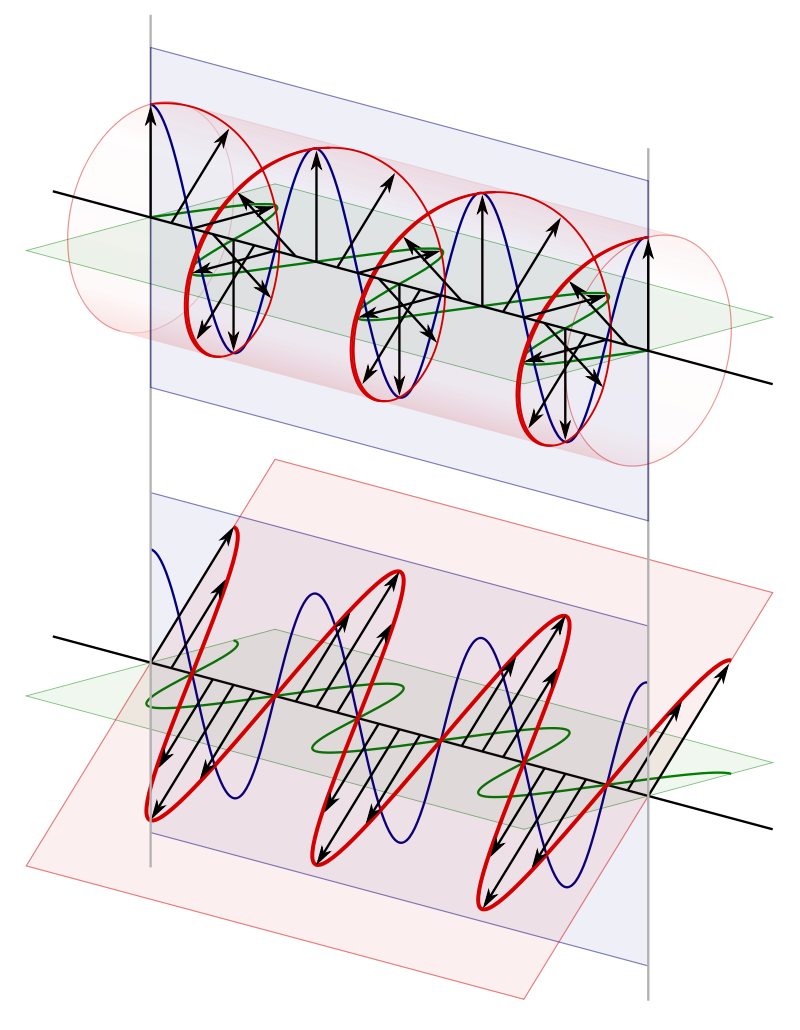
\includegraphics[width=0.4\textwidth]{refferenced_pic/qwp.png}
    \caption{Dependign on the initial polarization the quater-wave plate changes the polarization of the electric field to a circular (upper picture) or elliptical polarization (lower picture).
    The picture is taken from source \cite{qwp}.}
    \label{fig:qwp}
\end{figure}
\FloatBarrier
\subsection{Wollaston prism}
\label{sec:wollaston}
The probe beam polarization, after the detector crystal, carries all the information about the $\si{\tera\hertz}$-electric field strength.
Because its not possible to measure the polarization of the probe beam directly, it is necessary to split the probe beam into its two polarization components.
This happens with a wollaston prism, shown in figure \ref{fig:wollaston}.
It basically consist of two prism that are glued together.
The light that passes through the prism now refracts at the point where the two prsims touch.
From the fresnel equations it is possible to derive, that depending on the polarization of the light it gets refracted diffrently.
In the wollaston prism this means that the beam splits into a horizontal and a vertical polarized beam, with an angle of about $\SI{20}{\degree}$.
Its than possible to detect the insenity of both beams to derive the change in polarization that occured at the detector crystal. 
\begin{figure}
    \centering
    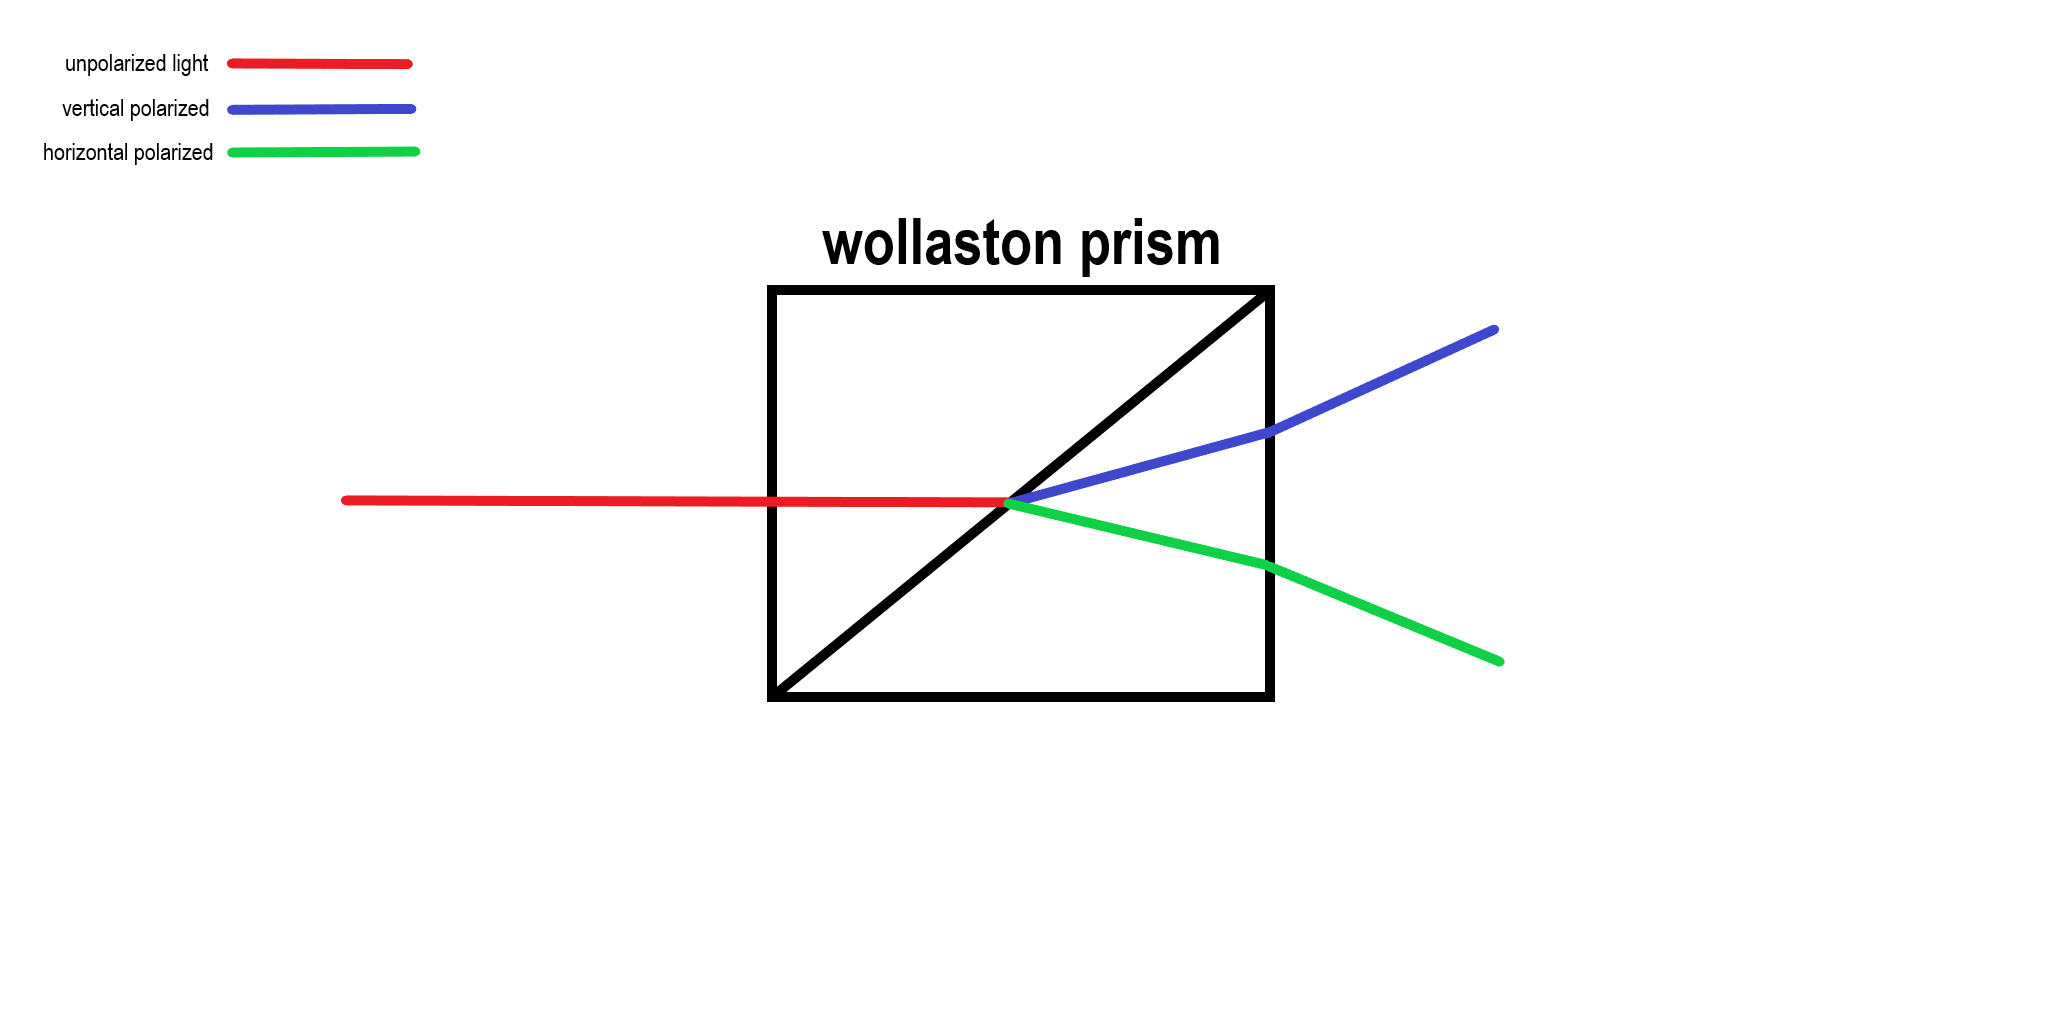
\includegraphics[width=0.7\textwidth]{refferenced_pic/wollaston.png}
    \caption{The picture shows a wollaston prism thorugh which an unpolarized beam passes.
    This beam refracts inside the prism which splits into two beams with perpindicular polarization.
    The two beams than leave the prism with an angle between them.}
    \label{fig:wollaston}
\end{figure}
\section{Time resolved THz spectroscopy}
\label{sec:time_domain}
To achieve a time resolved measurment of the $\si{\tera\hertz}$-pulse a delay stage is build into the setup.
With the delay stage the path length of the pump beam can be changed.
This way a time delay between pump pulse and probe pulse is achieved.
Because the velocity of electromagentic radiation in air is roughly the same as in a vacuum we can calculated the time delay   
\begin{equation}
    \Delta t = \frac{\Delta s}{c}
\end{equation}
with $c$ as the speed of ligth, and $\Delta s$ the diffrence in beam path.
The time resolved measurment now works by taking one measurment at delay stage position $s_1$, which corresponse to $t_1$.
Then the stage is moved to position $s_2$ this lengthens or shortens the beam path of the pump beam.
At stage position $s_2$ a new measurment is taken which corresponse to time $t_2$.
Now there is a time delay $\Delta t_{1-2} = t_1 - t_2$ between the two measurments.
This processes is repeated until the whole $\si{\tera\hertz}$-pulse is probed.

\section{Execution}
This section describes how the measurements were taken. 
It will be discussed what changes to the setup in figure \ref{fig:setup} are being made to achieve the wanted results.
\\\\
Before any measurements are taken the photodiodes have to be balanced.
For this a chopper is placed inside the probe beam, which modultes its frequency to $\SI{388}{\hertz}$.
The lock in amplifier gets triggered on that frequency, while its inputs are the $A$ and $B$ value of the two photodiodes.
It is necessary to move the stage to a point where $\si{\tera\hertz}$-pulse and probe pulse dont overlap, so that the polarization of the probe beam is not changed by the detector crystal.
Now the quater-wave plate is being rotated until the output of both photodiodes $A-B = 0$. 
This means the probe beam is circular polarized after the quater-wave plate, while it is not affected by the $\si{\tera\hertz}$ signal.
\subsection{Fluence measurments}
The goal of the fluence measurements is to determine the effect of diffrent pump fluences on the $\si{\tera\hertz}$ production.
For it is necessary to change the power of the pump beam before it hits the emitter crystal.
For that diffrent density filter are placed inside the beam path.
All that filter that were used can be seen in table \ref{tab:filters}.
The filters are placed inside a mount right after the chopper.
After the placementa the pump power is measured behind the filter.
Then the power meter is removed and a time resolved measurement \ref{sec:time_domain} of the pulse is taken.
After the measurement the filter is swapped out with another one and the process is started over until all possible fluences are measured.
\subsection{Electric field measurments}
To determine the electric field of the $\si{\tera\hertz}$ radiation it is necessary to measure the output of the photodiodes $A$ and $B$ seperatly aswell as there diffrence $A-B$.
Because just the maximum field strength is of particular interest just the greatest $A-B$ value is necessary to measure.
For this the delay stage is moved at the position of the greatest $A-B$ value and a measurement of the diffrence is taken.
This process has to be repeated for all pump power values that are wanted.
After all the diffrences are measured, $A$ and $B$ are measured seperatly.
The delay stage is moved to a position where there is no $\si{\tera\hertz}$-signal.
At this position the input of the lock in amplifier is changed to just one of the photodiodes outputs, either $A$ or $B$.
Because the sum $A+B$ is not affected by the $\si{\tera\hertz}$ electric field, it can be used to norm every difference.
So the seperatly measured values of $A$ and $B$ have to be measured just once.
After $A-B$ and $A$ and $B$ are measured the electric field can be calculated.
\subsection{Transmission measurments}
